\chapter{Methodologie}
Dit hoofdstuk beschrijft het proces van de implementatie van ons systeem. Een eerste sectie handelt over een bestaande implementatie, waarop ons systeem is gebaseerd. Een tweede sectie beschrijft onze eigen extensie van de code van Karpathy, meer specifiek hoe we LDA topic verdelingen gebruiken om extra semantische informatie toe te voegen. Een derde sectie gaat over onze implementatie van het eerder vernoemde gLSTM netwerk zoals voorgesteld door Jia \todo{reference?}. De laatste sectie beschrijft hoe wij een normalisatie hebben toegevoegd aan de beam search om zinnen te maken (zoals voorgesteld door Jia \todo{ref}).

\section{Startpunt Karpathy} \todo{Betere titel}
Het startpunt van onze implementatie is de code aangereikt door A. Karpathy op zijn github pagina. Die bevat een implementatie van het recurrente neurale netwerk beschreven in \todo{reference naar karpathy}, alsook een implementatie die gebaseerd is op \todo{reference vinyals}. Op basis hiervan hebben wij een aantal extensies ge\"implementeerd.
\subsection{Recurrent Neuraal Netwerk}
Een eerste implementatie waarvan we zijn vertrokken is beschreven in Karpathy\todo{ref!}. Hij beschrijft een systeem dat op basis van een afbeelding een beschrijvende zin genereert. Dit gebeurt in twee stappen. Eerst wordt de afbeelding door middel van een CNN omgezet naar een vector representatie. Deze vector dient vervolgens als input voor een recurrent neuraal netwerk.

\paragraph{Afbeeldingsrepresentatie}

\paragraph{Van afbeelding naar beschrijving}
De berekende vector representatie van de afbeelding dient als input voor een recurrent neuraal netwerk. Tijdens de training van het netwerk wordt op basis van de afbeelding, in combinatie met een speciale startvector die het begin van een zin aangeeft, het eerste woord voorspeld. Daarna wordt op basis van het eerste woord van de zin een voorspelling gemaakt voor het tweede woord. Dit proces herhaalt zich tot het einde van de zin bereikt is. Terugpropagatie op basis van stochastic gradient descent zorgt voor de juiste wijzigingen aan de gewichten van het netwerk. Een eenvoudige weergave dit proces is te zien op figuur \ref{fig:rnntraining}.

\begin{figure}[tb]
    \centering
    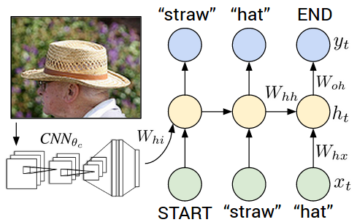
\includegraphics[width=0.5\linewidth]{Images/karpathy.PNG}
    \caption{Generatie van caption met recurrent neuraal netwerk}
    \label{fig:rnntraining}
\end{figure}

Het genereren van captions gebeurt op basis van beam search. Hierbij wordt op basis van de afbeelding een ranking gemaakt van de meest waarschijnlijke eerste woorden voor de zin. De eerste $n$ woorden dienen dan als startpunt van de voorspelling van het tweede woord. Over alle mogelijke sets van twee woorden wordt opnieuw een rangschikking gemaakt, waarvan de $n$ beste resultaten worden bijgehouden. Dit proces herhaalt zich tot elke vertakking van de zoekboom is onderzocht, waarna de beste gegenereerde zin wordt gebruikt als eindresultaat.


\subsection{Long Short Term Memory Netwerk}

\section{Toevoeging van LDA topicverdeling aan RNN}


\section{gLSTM}



\section{Normalizatie van beam search}